\section{Recolección}

%-------------------------------Recolección----------------------------------------------%
%-----------------------------Chcecar TT1------------------------

El proceso de recolección es parte fundamental del presente trabajo terminal, ya que permitió conformar el corpus necesario para llevar a cabo la etapa de entrenamiento, este proceso se llevo a cabo por etapas.

\begin{itemize}
	\item Seleccionar los sitios web
	\item Información a recolectar
	\item Análisis del sitio web
	\item Proceso de recolección
\end{itemize}

\subsection{Selección de sitios web}

El sitio web El Economista\footnote{https://www.eleconomista.com.mx/} contiene una sección llamada 
\textbf{Ranking de Medios Nativos Digitales}\footnote{https://www.eleconomista.com.mx/Ranking-de-Medios-Nativos-Digitales}, 
el cual muestra las estadísticas que realiza mes con mes acerca de los sitios de noticias web más consultados como se muestra en la Figura \textbf{\ref{fig:rank}}
\begin{figure}[H]
  \centering
  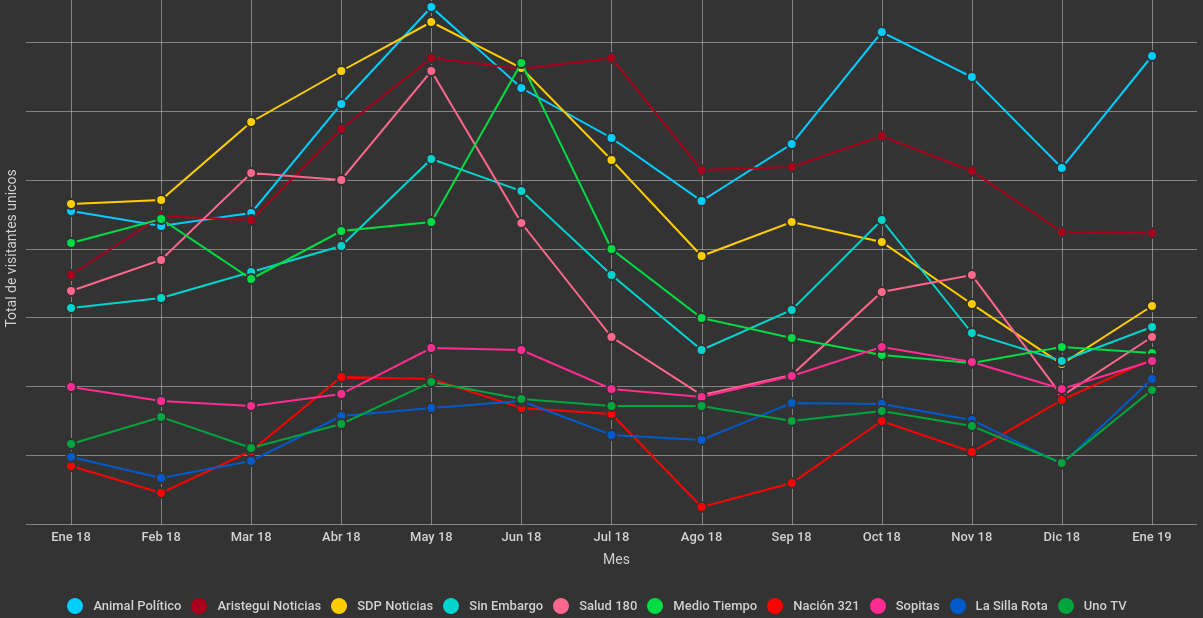
\includegraphics[scale=.28]{imagenes/Capitulo5/ranking.png}
  \caption{Ranking de sitios de noticias del periódo de enero del 2018 a enero del 2019.}
  \label{fig:rank}
\end{figure}

Con base en la Figura  se han seleccionado los diarios Aristegui Noticias, El Economista, La Jornada, La Prensa, Proceso, Sopitas y TV Azteca para recolectar noticias.

\Tlabel{c5:sitios}

\subsection{Información recolectada}

Se llevó a cabo un análisis acerca de la información que contiene cada una de las noticias y con base en ello se determinó recolectar la siguiente información:

\begin{itemize}
	\item URL de la noticia
	\item Título
	\item Fecha
	\item Sección
	\item Autor
	\item Descripción
	\item Noticia
\end{itemize}

Cabe destacar que no toda la información recuperada fue utilizada en el proceso de entrenamiento, sin embargo se considerarón los puntos anteriores ya que la mayor parte de las noticias cuentan con esa información.
%-----------------------------Chcecar TT1------------------------

%------------------------------------------- Listo
\subsection{Análisis de sitios web}

Una vez definida la información requerida de cada noticia se realizó un análisis sobre la estructura HTML de cada sitio web, con el fin de realizar expresiones \textit{XPath} quien permitie recorrer y procesar un documento XML, dado que cada sitio web cuenta con una estructura diferente, ha sido necesario realizar el análisis individual. Cabe mencionar que existen sitios los cuales realizan actualizaciones a su página, por esta razón cada dos meses se analizaban, con el fin de verificar que la estructura XML no cambiara.
\\
Una expresión \textit{XPath} de ruta permite buscar y seleccionar los distintos nodos de un documento XML(ver). En el siguiente Cuadro \ref{box:xmlEjemplo} se muestra un ejemplo con los elementos de una nota, los cuales son: \textbf{para} \textbf{de} \textbf{titulo} \textbf{texto}, en un documento XML estos son los nodos que conforman una nota.\\

\begin{mygraybox}[label={box:xmlEjemplo}]{Documento XML} 
<nota>\\
	<para>Daniel</para>\\
	<de>Andres</de>\\
	<titulo>Recordatorio</titulo>\\
	<texto>Recuerda despertar temprano.</texto>\\
</nota>
\end{mygraybox}

La expresión \textit{XPath} que permite extraer el contenido de la etiqueta \textbf{<texto> </texto>} se muestra en el Cuadro \ref{box:xpathEjemplo}: 

\begin{mygraybox}[label={box:xpathEjemplo}]{Expresión XPath} 
\textbf{/nota/texto/text()}
\end{mygraybox}

Para cada sitio web se crearon expresiones \textit{XPath} para recolectar el contenido.

%------------------------------------------- Listo
\subsection{Creación de recolectores}

Como se explicó en el capítulo 3 (ver\ref{c3:Crawler}) un \textit{Crawler} te permite descargar información de una página web, como se muestra en la Figura \ref{Fig:recoleccion}. La implementación en el trabajo terminal ha requerido diseñar 7 recolectores, uno por cada sitio web (ver \Tref{c5:sitios}{sitios web}). \\


\begin{figure}[H]
	\centering
	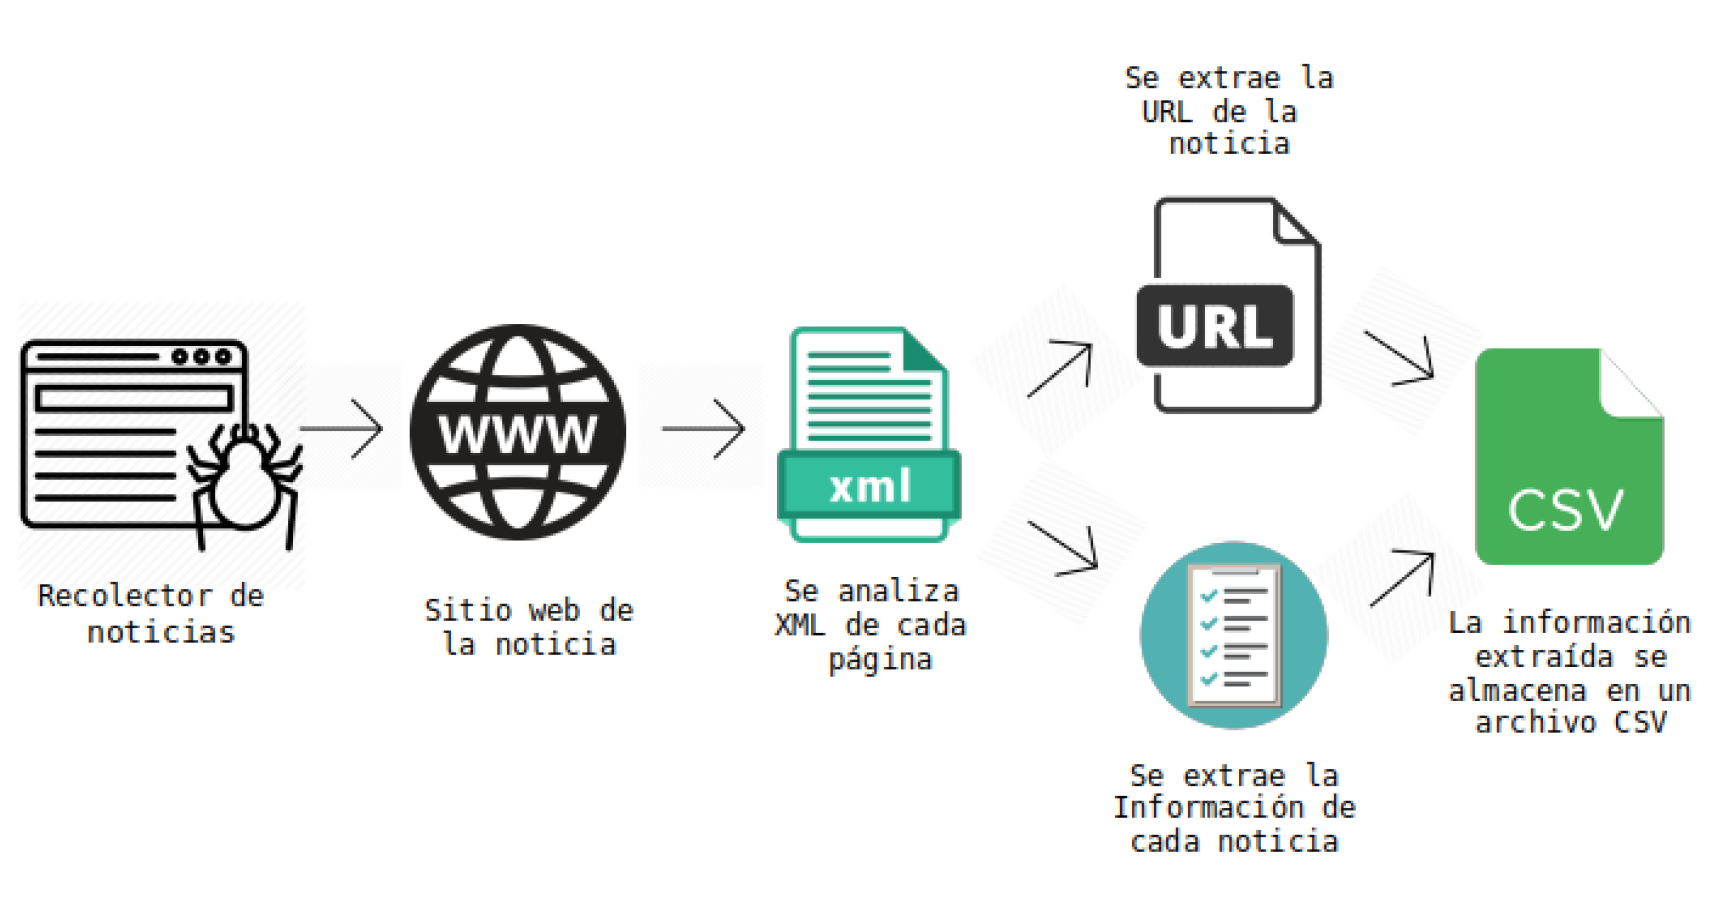
\includegraphics[scale=.2]{imagenes/Capitulo5/recoleccion.png}
	\caption{Proceso de recolección}
	\label{Fig:recoleccion}
\end{figure}

Para el desarrollo se ha utilizado el lenguaje de programación \textbf{Python3}, en conjunto con la librería \textbf{scrapycrawl}. Cabe destacar que las noticias recolectadas se almacenaron en un archivo CSV (ver\ref{}) con la estructura que se muestra en la Tabla \ref{tab:csv}, donde la primera fila (Encabezado) define los elementos de este archivo, además las filas consecuentes representan el contenido recolectado de cada noticia.\\

%\begin{mygraybox}[label={box:csv}]{Encabezado de un archivo CSV}
\begin{table}[H]
\centering
\resizebox{\columnwidth}{!}{
\begin{tabular}{|c |c |c |c |c |c |c}
\hline
\textbf{url}& \textbf{título}& \textbf{autor}& \textbf{fecha}& \textbf{descripción}& \textbf{noticia}\\
\cline{1-6}
url ejemplo 1& título ejemplo 1& autor ejemplo 1& fecha ejemplo 1& descripción ejemplo 1& noticia ejemplo1\\
\hline
url ejemplo 2& título ejemplo 2& autor ejemplo 2& fecha ejemplo 2& descripción ejemplo 2& noticia ejemplo2\\
\hline
\end{tabular}
}
\caption{Ejemplo de estructura de un archivo CSV}
\label{tab:csv}
\end{table}
%\end{mygraybox}

donde :
\begin{itemize}
	\item \textbf{url}: La dirección web donde se encuentra localizada la noticia 
	\item \textbf{título}: Encabezado de la noticia recolectada
	\item \textbf{autor}: Es el nombre de la persona que redacto la noticia o el nombre de la editorial
	\item \textbf{fecha}: Es la fecha en la cual la noticia ha sido publicada
	\item \textbf{descripción}: Es una idea general del contenido de la noticia. Cabe mencionar que no todas las noticias cuentan con una descripción
	\item \textbf{noticia}: Es la redacción realizada por el autor acerca de la noticia. Es de relevancia mencionar que este elemento más importante de los artículos decargados 
\end{itemize}

\subsection{Proceso de recolección de noticias}


Para el desarrollo de esta etapa, se recolectaron noticias de las secciones : \textbf{ciencia y tecnología}, \textbf{cultura}, \textbf{deportes}, \textbf{economía} y \textbf{política}, de los sitios web \textbf{Aristegui Noticias}, \textbf{El Economista}, \textbf{La Jornada}, \textbf{La Prensa}, \textbf{Proceso}, \textbf{Sopitas} y \textbf{TV Azteca}, durante el periodo de julio a septiembre cada cuatro días, con el fin de no tener noticias repetidas. El almacenamiento de las noticias se realizó en un directorio por sección, dentro de cada uno de estos se dividian las noticias recolectadas por sitio web. 
\\

Una vez finalizada la primera etapa de recolección, los resultados obtenidos por sección se muestran en la Figura  \ref{Fig:notseccionV1}.
%Mencionar como nombre primer corte de recolección y poner numero de noticias
\begin{figure}[H]
	\centering
	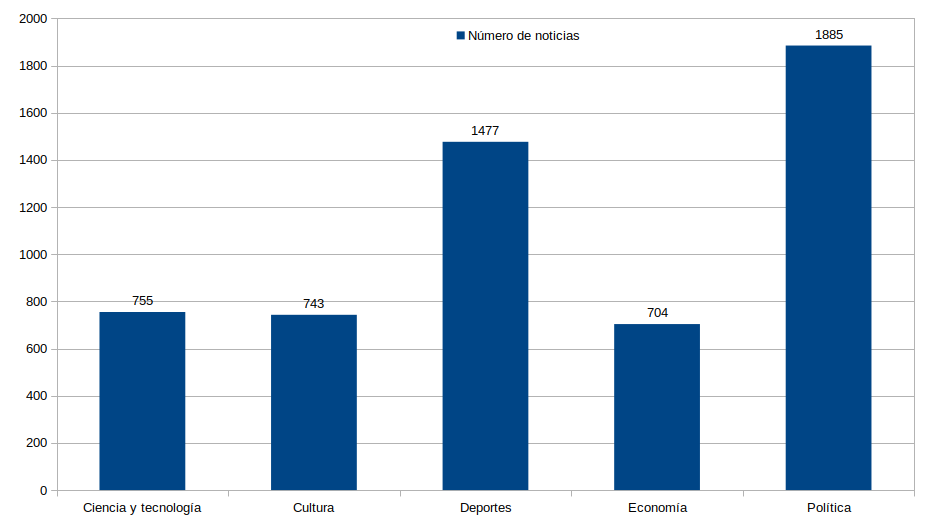
\includegraphics[scale=.6]{imagenes/Capitulo5/noticiasPorSeccionV1.png}
	\caption{Noticias recolectadas durante el primer corte.}
	\label{Fig:notseccionV1}
\end{figure}

Cabe destacar que el número de noticias no se encontraba balanceado debido a que no exite un gran número de sitios que publiquen noticias de cultura, por ello se decidió continuar con el proceso de recolección de noticias, con el fin de balancear el corpus y así los resultados obtenidos en la práctica mejoraron.
\\
Una vez finalizada la segunda etapa de recolección el número de noticias se muestra en la Figura \ref{Fig:notseccion}

\begin{figure}[H]
	\centering
	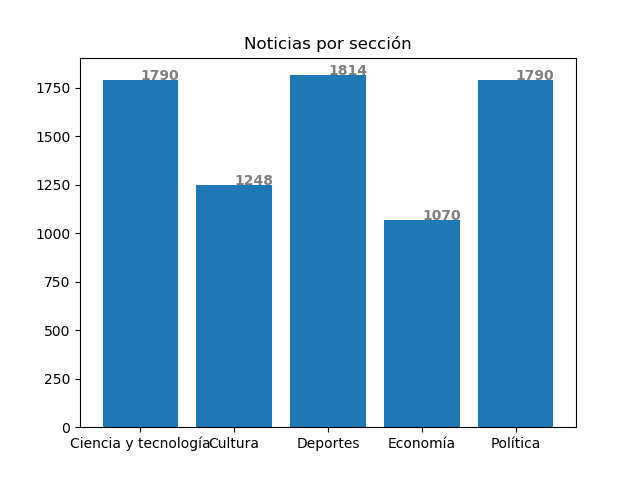
\includegraphics[scale=.6]{imagenes/Capitulo5/noticiasPorSeccion.png}
	\caption{Numero total de noticias recolectadas por sección.}
	\label{Fig:notseccion}
\end{figure}

Los noticias recuperadas por cada sitio web, se muestran en las siguientes Figuras.
\\

\begin{figure}[H]
	\centering
	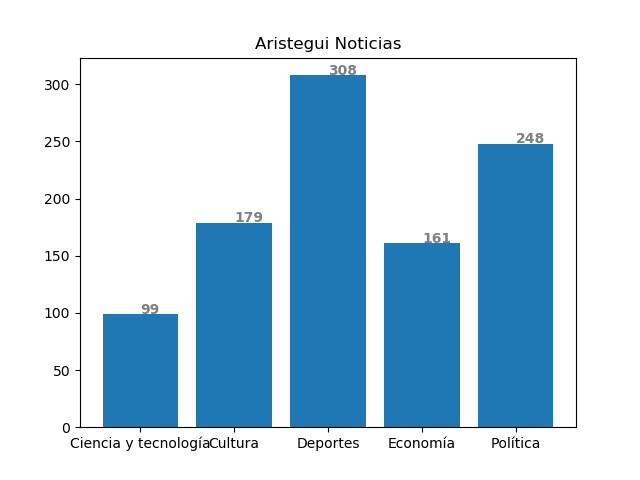
\includegraphics[scale=.45]{imagenes/Capitulo5/aristegui.png}
	\caption{Total de noticias recolectadas del sitio web de Aristegui Noticias}
	\label{Fig:notsitioaristegui}
\end{figure}

\begin{figure}[H]
	\centering
	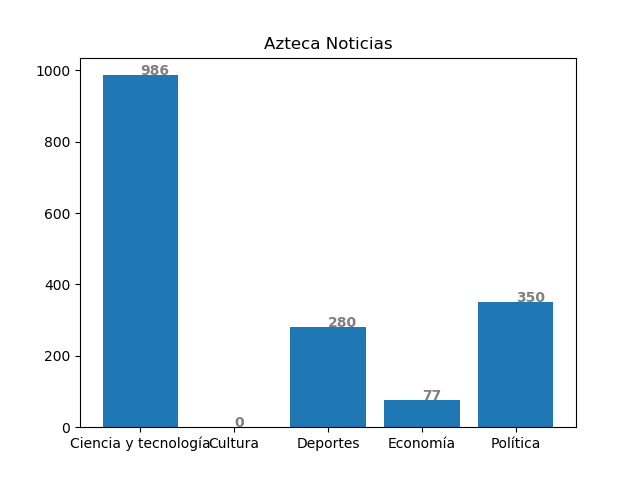
\includegraphics[scale=.45]{imagenes/Capitulo5/azteca.png}
	\caption{Total de noticias recolectadas del sitio web de Azteca Noticias}
	\label{Fig:notsitioazteca}
\end{figure}

\begin{figure}[H]
	\centering
	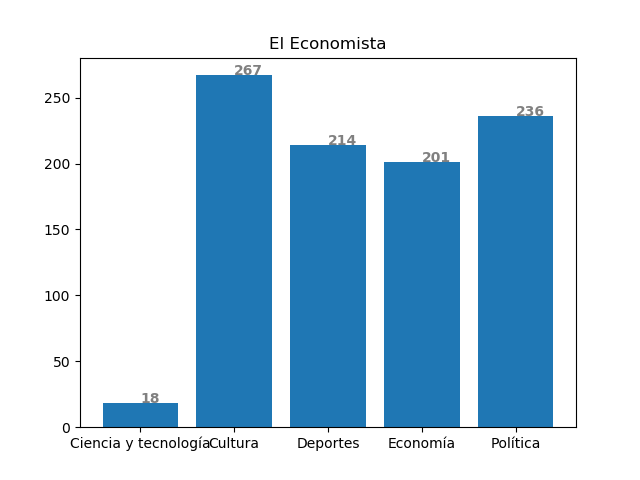
\includegraphics[scale=.45]{imagenes/Capitulo5/economista.png}
	\caption{Total de noticias recolectadas del sitio web de El Economista}
	\label{Fig:notsitioeconomista}
\end{figure}

\begin{figure}[H]
	\centering
	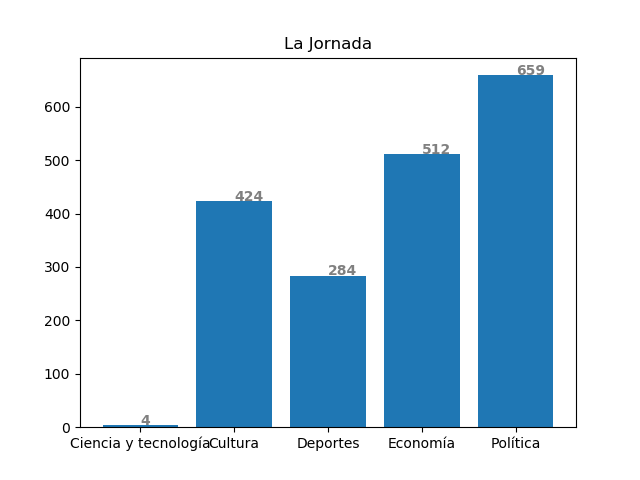
\includegraphics[scale=.45]{imagenes/Capitulo5/jornada.png}
	\caption{Total de noticias recolectadas del sitio web de La Jornada}
	\label{Fig:notsitiojornada}
\end{figure}

\begin{figure}[H]
	\centering
	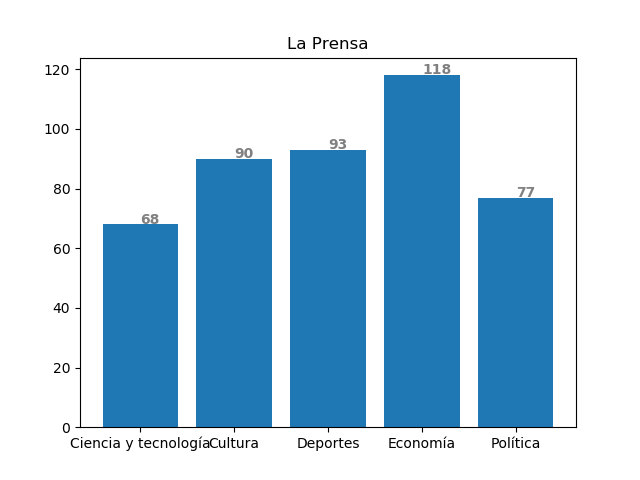
\includegraphics[scale=.45]{imagenes/Capitulo5/prensa.png}
	\caption{Total de noticias recolectadas del sitio web de La Prensa}
	\label{Fig:notsitioprensa}
\end{figure}

\begin{figure}[H]
	\centering
	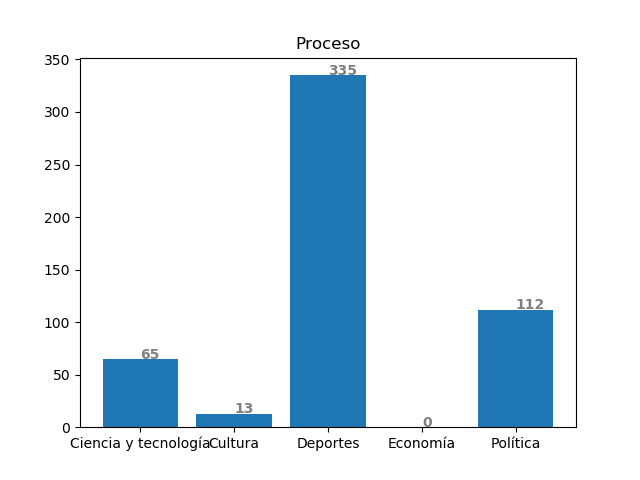
\includegraphics[scale=.45]{imagenes/Capitulo5/proceso.png}
	\caption{Total de noticias recolectadas del sitio web de Proceso}
	\label{Fig:notsitioproceso}
\end{figure}

\begin{figure}[H]
	\centering
	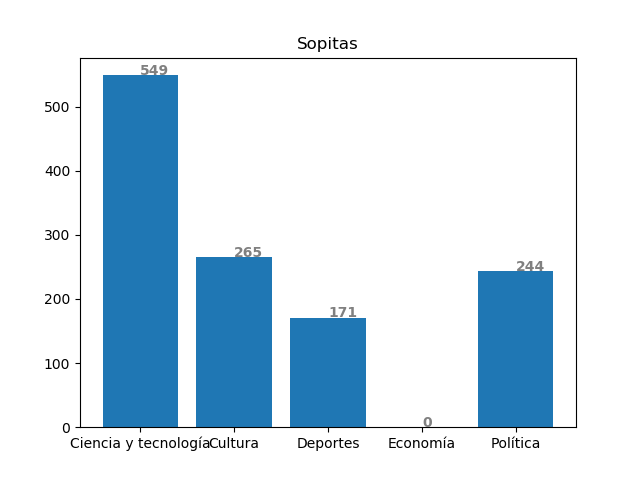
\includegraphics[scale=.45]{imagenes/Capitulo5/sopitas.png}
	\caption{Total de noticias recolectadas del sitio web de Sopitas}
	\label{Fig:notsitiosopitas}
\end{figure}

Una vez concluida la recolección de noticias se procedió con el balanceo de noticias quedando un total de 700 noticias por sección.	